\documentclass[letterpaper,12pt]{article}
\usepackage[section=1.2]{mathhw}
\usepackage{siunitx}
\usepackage{chemformula}
\usepackage{pgfplots}

\pgfplotsset{
  compat=newest,
  histogram/.style={
    axis lines=middle,
    axis line style={-Latex},
    xlabel near ticks,
    ylabel near ticks,
    xtick=data,
    xticklabel style={/pgf/number format/fixed},
    yticklabel style={/pgf/number format/fixed},
    area style
  }
}

\begin{document}

\maketitle

\begin{enumerate}
  \item[11.]
    The accompanying specific gravity values for various wood types used in construction appeared in the article ``Bolted Connection Design Values Based on European Yield Model'' (\textit{J. of Structural Engr., 1993: 2169-2186}):
    \begin{center}
      \begin{tabular}{l l l l l l l l l}
        .31 & .35 & .36 & .36 & .37 & .38 & .40 & .40 & .40 \\
        .41 & .41 & .42 & .42 & .42 & .42 & .42 & .43 & .44 \\
        .45 & .46 & .46 & .47 & .48 & .48 & .48 & .51 & .54 \\
        .54 & .55 & .58 & .62 & .66 & .66 & .67 & .68 & .75
      \end{tabular}
    \end{center}
    Construct a stem-and-leaf display using repeated stems, and comment on any interesting features of the display.
    \begin{center}
      \begin{tabular}{c | c c c c c c c c c c c c c c c c c c c}
        % Stem & \multicolumn{19}{l}{Leaf} \\
        % \hline
        3 & 1 & 5 & 6 & 6 & 7 & 8 \\
        4 & 0 & 0 & 0 & 1 & 1 & 2 & 2 & 2 & 2 & 2 & 3 & 4 & 5 & 6 & 6 & 7 & 8 & 8 & 8 \\
        5 & 1 & 4 & 4 & 5 & 8 \\
        6 & 2 & 6 & 6 & 7 & 8\\
        7 & 5 \\
        \multicolumn{20}{r}{Key: 1 | 2 = 0.12}
      \end{tabular}
    \end{center}
    The display has one peak at stem 4. It suggests that a typical value is in stem 4, perhaps 0.42. The data is not quite symmetric since the larger values tend to be more stretched out than the smaller ones. There is a bit of a gap between the largest value and the rest of the data (0.68 versus 0.75).
  \item[12.]
    The accompanying summary data on \ch{CeO2} particle sizes (nm) under certain experimental conditions was read from a graph in the article ``Nanoceria – Energetics of Surfaces, Interfaces and Water Adsorption'' (\textit{J. of the Amer. Ceramic Soc.}, 2011: 3992–3999):
    \begin{center}
      \begin{tabular}{>{\itshape}l c c c c c}
        Class & 3.0--<3.5 & 3.5--<4.0 & 4.0--<4.5 & 4.5--<5.0 & 5.0--<5.5 \\
        Frequency & 5 & 15 & 27 & 34 & 22 \\
        Relative frequency & .038 & .115 & .206 & .281 & .168 \\
        Density & .019 & .058 & .103 & .141 & .084 \\
        \hline
        Class & 5.5--<6.0 & 6.0--<6.5 & 6.5--<7.0 &  7.0--<7.5 & 7.5--<8.0 \\
        Frequency & 14 & 7 & 2 & 4 & 1 \\
        Relative frequency & .107 & .054 & .015 & .031 & .008 \\
        Density & .535 & .027 & .008 & .016 & .004
      \end{tabular}
    \end{center}
    \begin{enumerate}
      \item[a.]
        What proportion of the observations are less than 5?
        \begin{align*}
          5 + 15 + 27 + 34 &= 81 \\
          81 + 22 + 14 + 7 + 2 + 4 + 1 &= 131 \\
          \frac{81}{131} \approx 0.618 \approx 61.8\%
        \end{align*}
      \item[b.]
        What proportion of the observations are at least 6?
        \begin{align*}
          7 + 2 + 4 + 1 &= 14 \\
          5 + 15 + 27 + 34 + 22 + 14 + 14 &= 131 \\
          \frac{14}{131} \approx 0.107 \approx 10.7\%
        \end{align*}
      \item[c.]
        Construct a histogram with relative frequency on the vertical axis and comment on interesting features. In particular, does the distribution of particle sizes appear to be reasonably symmetric or somewhat skewed? [\textit{Note}: The investigators fit a lognormal distribution to the data; this is discussed in Chapter 4.]
        \begin{center}
          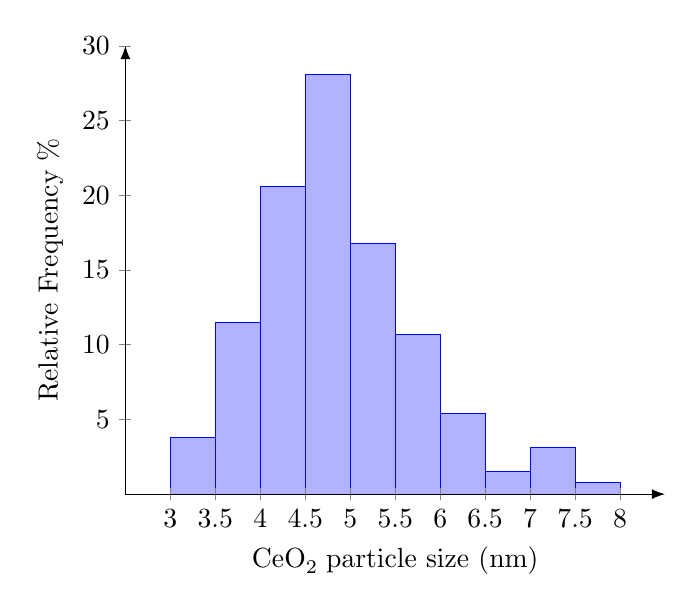
\begin{tikzpicture}
            \begin{axis}[
              histogram,
              ymax=30,
              xlabel={\ch{CeO2} particle size (nm)},
              ylabel={Relative Frequency \%},
              xtick distance=0.5,
              ytick distance=5,
              enlarge x limits=0.1,
            ]
              \addplot+[
                ybar interval,
                y filter/.code={\pgfmathparse{#1*100}\pgfmathresult}
              ] plot coordinates {
                (3.0, 0.038) (3.5, 0.115) (4.0, 0.206) (4.5, 0.281) (5.0, 0.168)
                (5.5, 0.107) (6.0, 0.054) (6.5, 0.015) (7.0, 0.031) (7.5, 0.008)
                (8.0, 0)
              };
            \end{axis}
          \end{tikzpicture}
        \end{center}
        The histogram rises fairly smoothly to a major peak, and then declines. The decline has a small peak towards the end. The histogram extends a bit more on the right (towards large values) than it does on the left. Thus, there is a positive skew.
      \item[d.]
        Construct a histogram with density on the vertical axis and compare to the histogram in (c).
        \begin{center}
          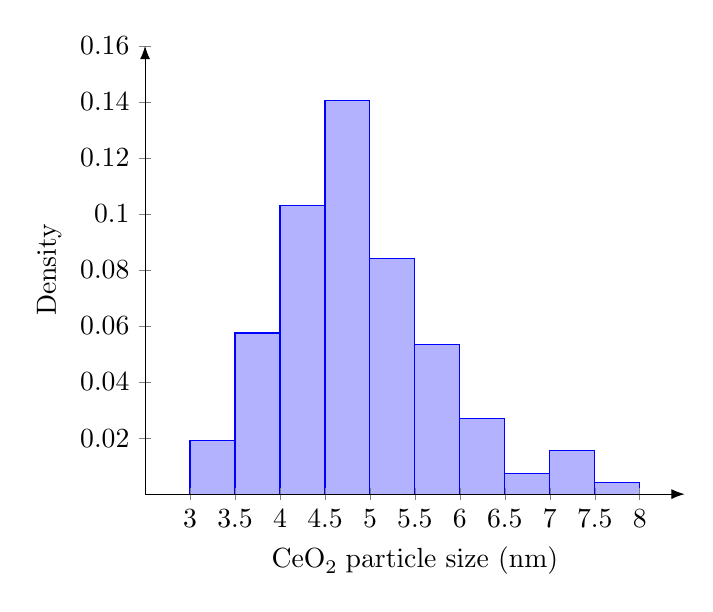
\begin{tikzpicture}
            \begin{axis}[
              histogram,
              ymax=0.16,
              xlabel={\ch{CeO2} particle size (nm)},
              ylabel={Density},
              xtick distance=0.5,
              ytick distance=0.02,
              enlarge x limits=0.1,
            ]
              \addplot+[
                ybar interval,
                y filter/.code={\pgfmathparse{#1/2}\pgfmathresult}
              ] plot coordinates {
                (3.0, 0.038) (3.5, 0.115) (4.0, 0.206) (4.5, 0.281) (5.0, 0.168)
                (5.5, 0.107) (6.0, 0.054) (6.5, 0.015) (7.0, 0.031) (7.5, 0.008)
                (8.0, 0)
              };
            \end{axis}
          \end{tikzpicture}
        \end{center}
        The histogram is identical to the one in (c). This is because all the classes have the same width (2). Thus, the vertical axis of (d) is simply scaled down by a factor of 2.
    \end{enumerate}
  \item[17.]
    The accompanying data came from a study of collusion in bidding within the construction industry (``Detection of Collusive Behavior,'' \textit{J. of Construction Engr. and Mgmnt}, 2012: 1251–1258).
    \begin{center}
      \begin{tabular}{S[table-format=2.0]S[table-format=2.0]}
        \textbf{No. Bidders} & \textbf{No. Contracts} \\
        2 & 7 \\
        3 & 20 \\
        4 & 26 \\
        5 & 16 \\
        6 & 11 \\
        7 & 9 \\
        8 & 6 \\
        9 & 8 \\
        10 & 3 \\
        11 & 2
      \end{tabular}
    \end{center}
    \begin{enumerate}
      \item[a.]
        What proportion of the contracts involved at most five bidders? At least five bidders?
      \item[b.]
        What proportion of the contracts involved between five and 10 bidders, inclusive? Strictly between five and 10 bidders?
      \item[c.]
        Construct a histogram and comment on interesting features.
    \end{enumerate}
  \item[19.]
    The number of contaminating particles on a silicon wafer prior to a certain rinsing process was determined for each wafer in a sample of size 100, resulting in the following frequencies:
    \begin{center}
      \begin{tabular}{
        >{\itshape}l
        S[table-format=2.0]
        S[table-format=2.0]
        S[table-format=2.0]
        S[table-format=2.0]
        S[table-format=2.0]
        S[table-format=2.0]
        S[table-format=2.0]
        S[table-format=2.0]
      }
        Number of particles & 0 & 1 & 2 & 3 & 4 & 5 & 6 & 7 \\
        Frequency & 1 & 2 & 3 & 12 & 11 & 15 & 18 & 10 \\
        Number of particles & 8 & 9 & 10 & 11 & 12 & 13 & 1 \\
        Frequency & 12 & 4 & 5 & 3 & 1 & 2 & 1
      \end{tabular}
    \end{center}
    \begin{enumerate}
      \item[a.]
        What proportion of the sampled wafers had at least one particle? At least five particles?
      \item[b.]
        What proportion of the sampled wafers had between five and ten particles, inclusive? Strictly between five and ten particles?
      \item[c.]
        Draw a histogram using relative frequency on the vertical axis. How would you describe the shape of the histogram?
    \end{enumerate}
  \item[22.]
    How does the speed of a runner vary over the course of a marathon (a distance of 42.195 km)? Consider determining both the time to run the first 5 km and the time to run between the 35-km and 40-km points, and then sub-
    tracting the former time from the latter time. A positive value of this difference corresponds to a runner slowing down toward the end of the race. The accompanying histogram is based on times of runners who participated in several different Japanese marathons (``Factors Affecting Runners’ Marathon Performance,'' \textit{Chance, Fall}, 1993: 24–30).

    What are some interesting features of this histogram? What is a typical difference value? Roughly what proportion of the runners ran the late distance more quickly than the early distance?

    \begin{center}
      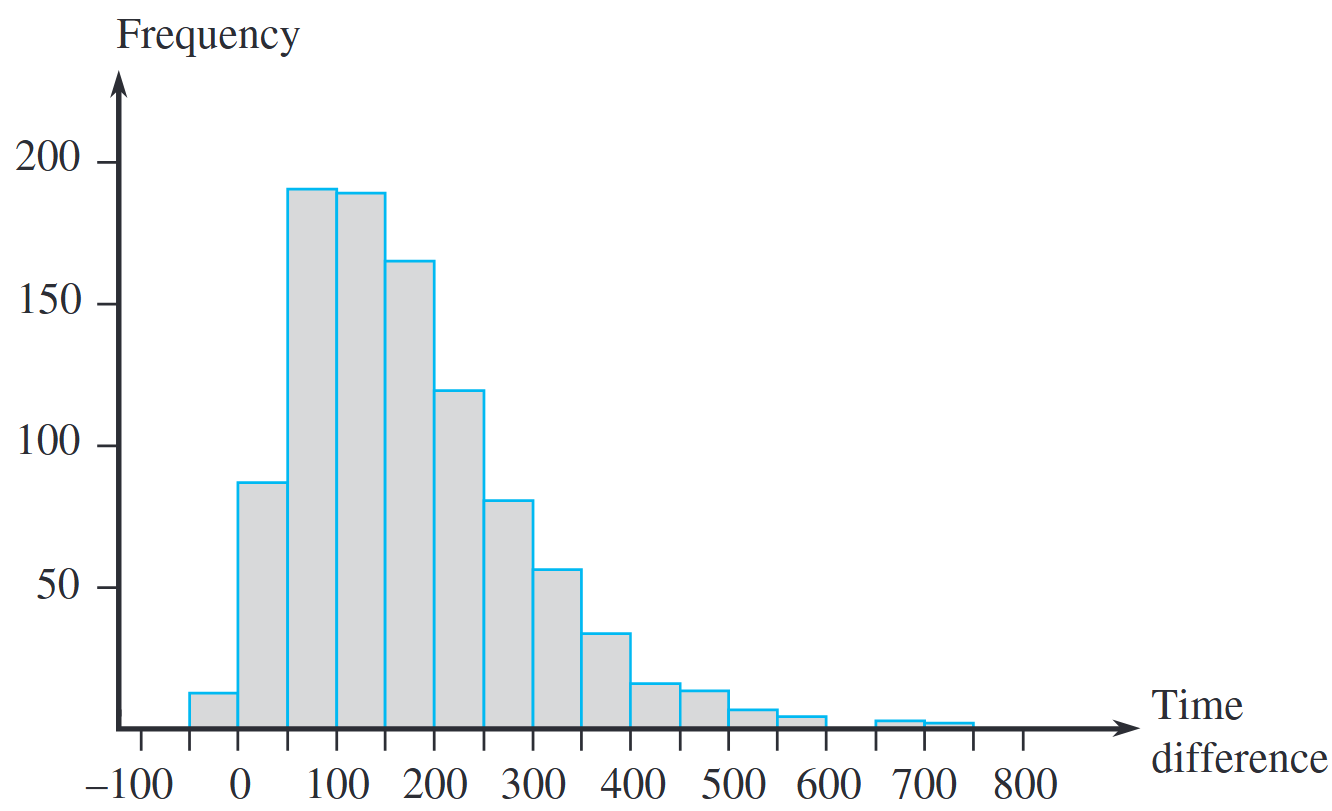
\includegraphics[scale=0.3]{../resources/01_02_22_01.png}
    \end{center}
\end{enumerate}

\end{document}
